\documentclass[a4paper,11pt]{article}

% Used packages
\usepackage[utf8]{inputenc}
\usepackage{geometry}
\usepackage{graphicx}
\usepackage{multicol}
\usepackage[compact]{titlesec}
\usepackage[hidelinks]{hyperref}
\usepackage{eso-pic}
\usepackage{xcolor}
\usepackage{lmodern}
\usepackage{contour}

% Document formatting
\geometry{margin=1in}
\titlelabel{\thetitle.\quad}
\setcounter{secnumdepth}{5}
%\frenchspacing
\titlespacing*{\section} {0pt}{3.5ex plus 0.5ex minus .15ex}{2.3ex plus .2ex}
\titlespacing*{\subsection} {0pt}{3.25ex plus 0.5ex minus .15ex}{1.5ex plus .2ex}
\titlespacing*{\subsubsection} {0pt}{3.0ex plus 0.5ex minus .15ex}{1.0ex plus .2ex}
\setlength{\parskip}{0pt}
\setlength{\parsep}{0pt}
\setlength{\headsep}{0pt}
\setlength{\topskip}{0pt}
\setlength{\topmargin}{0pt}
\setlength{\topsep}{0pt}
\setlength{\partopsep}{0pt}

\newcommand\BackgroundIm{
\put(0,0){
\parbox[b][\paperheight]{\paperwidth}{%
\vfill
\centering
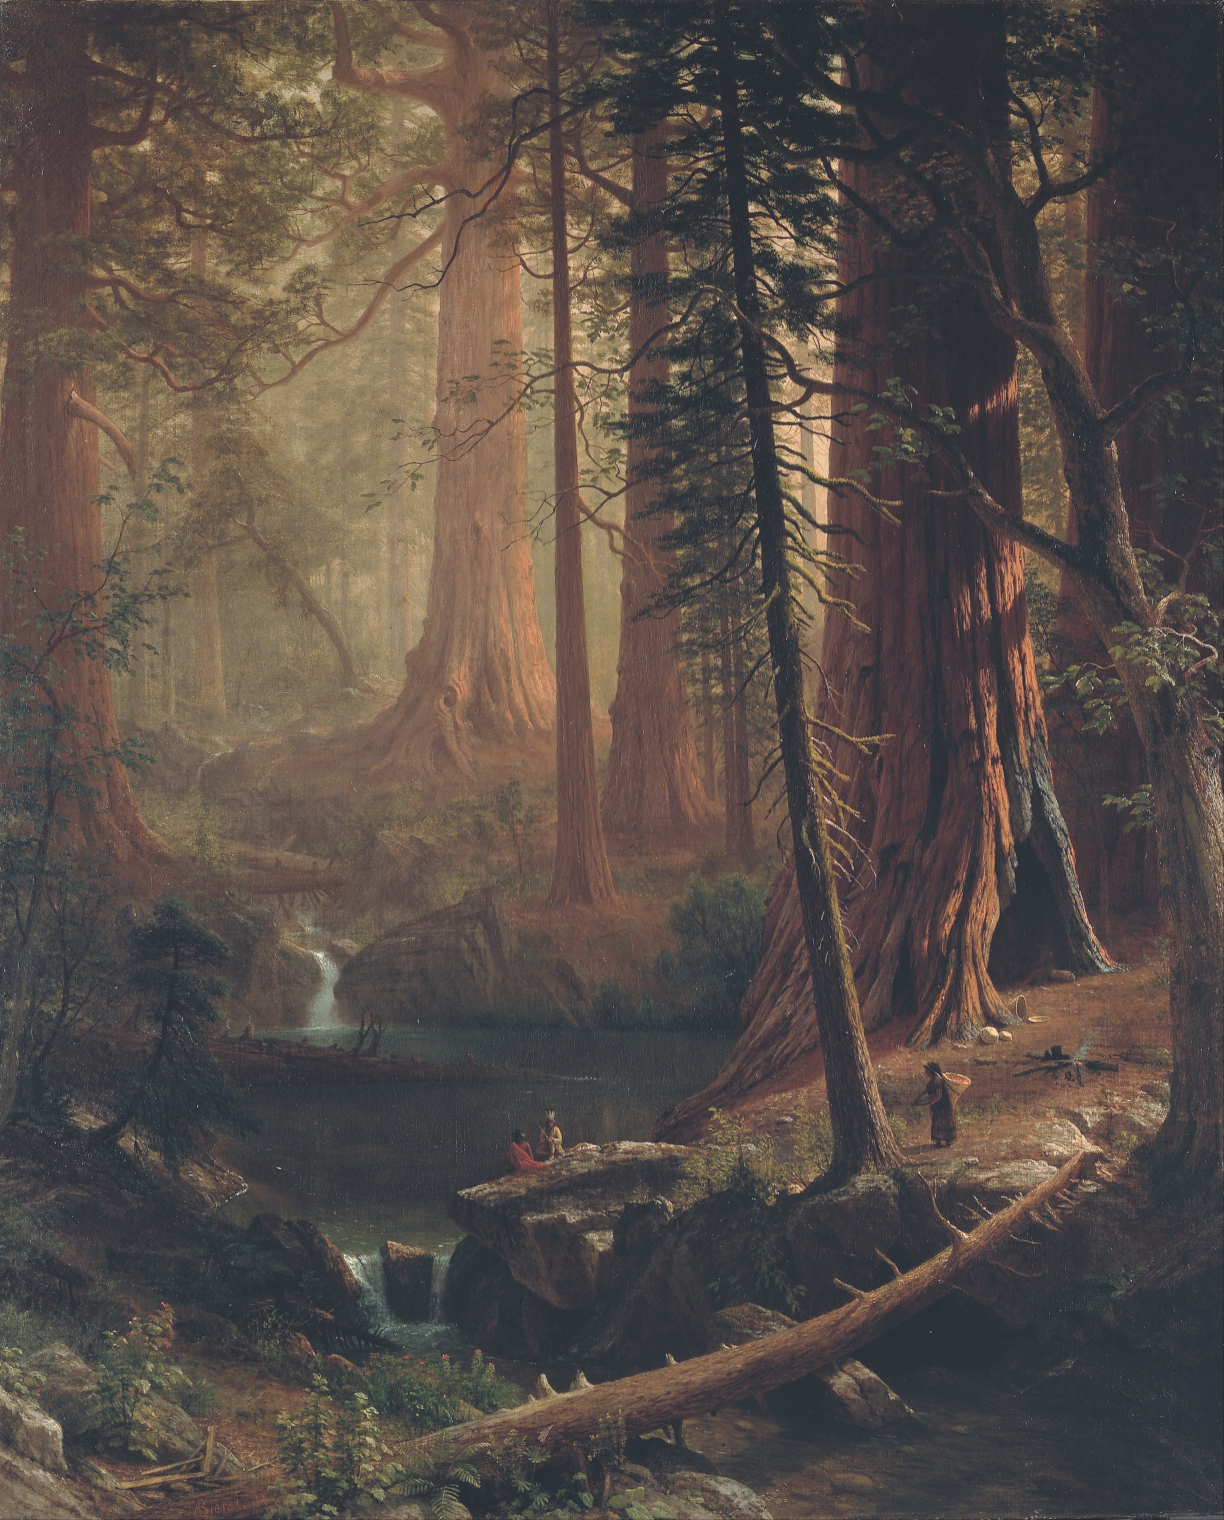
\includegraphics[height=\paperheight,width=\paperwidth, trim=2cm 2cm 2cm 2cm]{Bierstadt.jpg}%
\vfill
}}}

\contourlength{1pt}
\contournumber{5} 

% Opening
\font\titlefont=cmr12 at 40pt
\title{%
    \textbf{\titlefont Epitome} \\
        \large  An instrument built for change}
\author{Georgios Mavropalias$^{1}$, Panagiotis Tokmakidis$^{1}$, Pavlos Boudagidis$^{1}$}
\date{}

\begin{document}

\begin{titlepage}
\centering
\AddToShipoutPicture*{\BackgroundIm}
{\bfseries\Huge\color{white} \contour{black}{The Democracy Foundation}\\}
\vspace*{\fill}
\begin{figure*}[hb]
\centering
\resizebox{100mm}{!}{\input{wreath2.pdf_tex}}
\label{TDFlogoInv}
\end{figure*}
\vspace*{\fill}
\begin{flushleft}
{\bfseries\fontsize{2.5cm}{2cm}\selectfont\color{white} \contour{black}{Epitome}\\}  
\end{flushleft}
\begin{flushleft}
{\bfseries\fontsize{1cm}{2cm}\selectfont\color{white} \contour{black}{An instrument built for change}\\}  
\end{flushleft}
\vspace*{\fill}
\begin{flushright}
\selectfont\color{white} \contour{black}{Last updated: \today}
\end{flushright}

\end{titlepage}
\footnotetext[1]{\textbf{The Democracy Foundation} - \url{http://democracy.foundation/} \\


\includegraphics[height=10.0mm]{CC.jpg} \\

This work is licensed under a \href{http://creativecommons.org/licenses/by-sa/4.0/}{Creative Commons Attribution-ShareAlike 4.0 International License}.
}

\maketitle

\begin{multicols}{2}

\section{Introduction} \label{introduction}

Humanity faces challenges of global scale and accelerating impact that call for an immediate and effective plan of action to halt their expansion and reverse their effects on both our species and the environment. However, our current system of governance does not seem adequately equipped to find solutions, and in some cases it even exacerbates them. Legislators and representatives are still constrained by time, location, and space, with only a few hundred able to take part in decision-making at a time, and that itself is a time-consuming and inefficient process.

The creation of the internet brought along the promise of mass deliberation and collaboration by overcoming our physical barriers, but this promise remains unfulfilled. Proponents of the idea have envisioned that the internet would one day transform local, national, and even global governance and connect millions that would crowdsource solutions to humanity's problems. However, having conversations among thousands of users online and trying to reach consensus is impossible, despite the technological leaps in progress. The need still exists for a system of governance that will be able to seamlessly detect issues and create solutions, while not being affected by restraints of location, time, and space. Moreover, large participation should not impair the process, but improve the outcome.

For that reason, we introduce a new governance system that will render mass deliberation and effective issue-based consensus decision-making possible, without the need of representatives or intermediates, applied via ``Epitome'', a free and open source online platform. The platform features subsystems that dynamically scale according to the active population, protect from abuse and exploitation, as well as adjust to the urgency of each issue and the unique situations that emerge during the deliberation process.

We propose two implementation models, as will be described henceforth. The first is a worldwide expert community, composed of academics and researchers, that will enable the identification and solution-proposal of global challenges. Due to the fact that the global challenges that we face today are complex, comprised of many individual sub-components, and span across many fields of knowledge, it is impossible for a few hundred lawmakers or ambassadors to keep up with all the global incidents and the latest research in each field. The implementation of our system constituted by academics, will ensure that the most knowledgeable individuals can effectively identify and propose solutions.

The second implementation is on a national level. Using the platform, citizens will be able to deliberate and propose solutions to issues they detect in their societies, in the municipal, provincial, and national levels, while the platform will automatically adjust according to the nature and urgency of each issue. Additionally, the system could also work in conjunction with a delegative democracy model where elected experts would propose solutions to the most critical issues reported, and would submit them as referendums towards the entire population.

\subsection{Governance system} \label{governance}

The greatest challenge when it comes to building consensus in governance is not voting, but deliberation. An unresolved obstacle is the inability of hundreds or thousands of people deliberating simultaneously in an effective manner. So far, the methods used for online written conversation are underdeveloped. Typically, websites arrange replies in the same line, or nested underneath. This can work to some degree if there are a few hundred comments, but once thousands of people come together it is impossible to follow the discussion. Moreover, having administrators moderate user submissions or even give them the exclusive right to create proposals is an exploitable vulnerability prone to abuse of power and corruption. Our proposed governance system addresses the issues listed above innovatively, via a free and open source online platform.

We introduce a responsive platform named ``Epitome'', in which the individual proposals are subjected to peer-evaluation and cultivation without the need for intermediate persons monitoring or moderating the process. Additionally, in order for a proposal or a referendum to take place, there must be an issue that needs addressing. Instead of creating generic proposals, users are able to report issues, support them with evidence, submit proposals to those issues, and finally vote on what they deem a viable solution. Users are thus transformed into numerous issue detectors and a powerful solution-crowdsourcing force.

Even though the underlying mechanisms described below are complex in nature, users are introduced to an intuitive and friendly environment without needing to know the background workings.

\section{Analysis} \label{analysis}

\subsection{Values} \label{values}

In the following description, the values enclosed in braces \{\} are enabled by default, but they are not fixed nor final. Communities are able to configure them according to their size and needs.

Anonymity in the different aspects of the platform can be configured as well, with some communities choosing to have the processes of issue submission and proposal collaboration \{anonymous\}.

In each community, all values can be configured upon installation or modified later on, by the users themselves, via opening an issue and reaching consensus on the preferred value.

\subsection{Elements} \label{elements}

The four main element types of the platform are issues, evidence, proposals and referendums. Issues are, as their name suggests, issues submitted by users that require addressing. Evidence is the constituent element of an issue, providing relevant information. Proposals are suggested solutions to those issues, developed through a deliberation process. Referendums are proposals that reached a mature stage, and are now available for voting by the entire community. All submitted elements are static, meaning their information cannot change, to provide a reference point which users can cite in the future.

\section{Submission system} \label{submissionsystem}

\subsection{Cycles} \label{cycles}

In order to prevent excessive numbers of submissions, users are not able to directly submit elements towards the entire community. The subsystem of “Cycles” is a process through which an issue or a proposal is submitted to a small population sample, and if it is supported by that portion, it is then promoted to a higher cycle level, with a greater population segment.

Each cycle is a randomly selected subgroup of the entire population, organized to enable an easier overview and cultivation of the submitted elements. Cycles are arranged in cycle levels, and each of those levels contains 100\% of the registered population split equally in cycles. While each level has a different number of cycles, the capacity of each cycle adjusts so that their aggregate percentage is always 100\%. Each user is part of one cycle in each level.

The only cycle level a user can submit a proposal or issue to is the bottom one. If their submission is well-supported, it is promoted to the next level, which includes cycles of larger population percentage. If the proposal reaches the top level, and receives adequate support, it is converted to a referendum. Similarly, if an issue reaches the top level and receives adequate support, it is then exhibited to the entire population.

The number of cycles \{automatically\} adjusts according to the total number of registered users. The top level consists of \{10\} cycles that each contain \{10\%\} of the total population. Each level below contains \{$\frac{1}{3}$\} of the population of the previous-level cycles, and it is accordingly divided into \{3\} times the number of cycles. The addition of levels continues until the cycles in the bottom level contain \{less\} than \{1 thousand\} users. Using those values, a community with 1 thousand users will have only 1 level (with 10 cycles of 100 people each) while a community of 1 million users will contain 6 levels.

Cycles \{continuously\} check the active population and distribute the users evenly, to prevent having one cycle being at capacity and another one empty. Both cycles and their levels, are not active by default, but they activate as participation increases. A cycle \{must\} reach at least \{10\%\} of its capacity before another one is enabled, to prevent users from being too spread in the case of low participation. In order for a level to be activated, \{10\%\} of the total cycles that are contained at \{2\} levels below must be already active. Therefore, even though a community may have many levels, they remain inactive if participation is low.

If the platform is configured to check for the location of a user (e.g. a country), it would attempt to evenly distribute users from the same location or region to different cycles to prevent the formation of power groups. Additionally, each cycle, even in different levels, contains \{a new, random\} sample, meaning users who were part of a cycle in a specific level will not necessarily be in the same cycle again in a higher level. Therefore, the platform always strives to provide a random but representative sample of the entire community in each cycle. Every user \{can\} view any cycle at any level, but \{can only\} contribute to the ones they are assigned to.

\subsection{Capital} \label{capital}

There \{is\} a time limit after the submission of an element before a user can submit a new one. With the “Capital” subsystem, a user can make a maximum of \{1\} submission at all times, even if they have not submitted anything new for multiple renewal terms. This submission capital renewal rate, although configurable, is by default proportionate to the number of users present within a cycle. The \{number of users\} in a \{cycle\} is then converted to \{seconds\}, and that time period is the time a user has to wait between submissions, with a minimum of \{10 minutes\}. 

\subsection{The 33-60 principle} \label{principle}

The ``33-60'' principle describes the required condition of at least \{33\%\} of the active population reaching \{60\%\} agreement in a voting, so as to be considered accepted. Having a super-majority level of \{60\%\}, protects against a 51-49 split decision phenomenon and ensures that there is adequate support, whereas the required minimum of \{33\%\} of the active population ensures sufficient representation.

\begin{figure*}
\centering
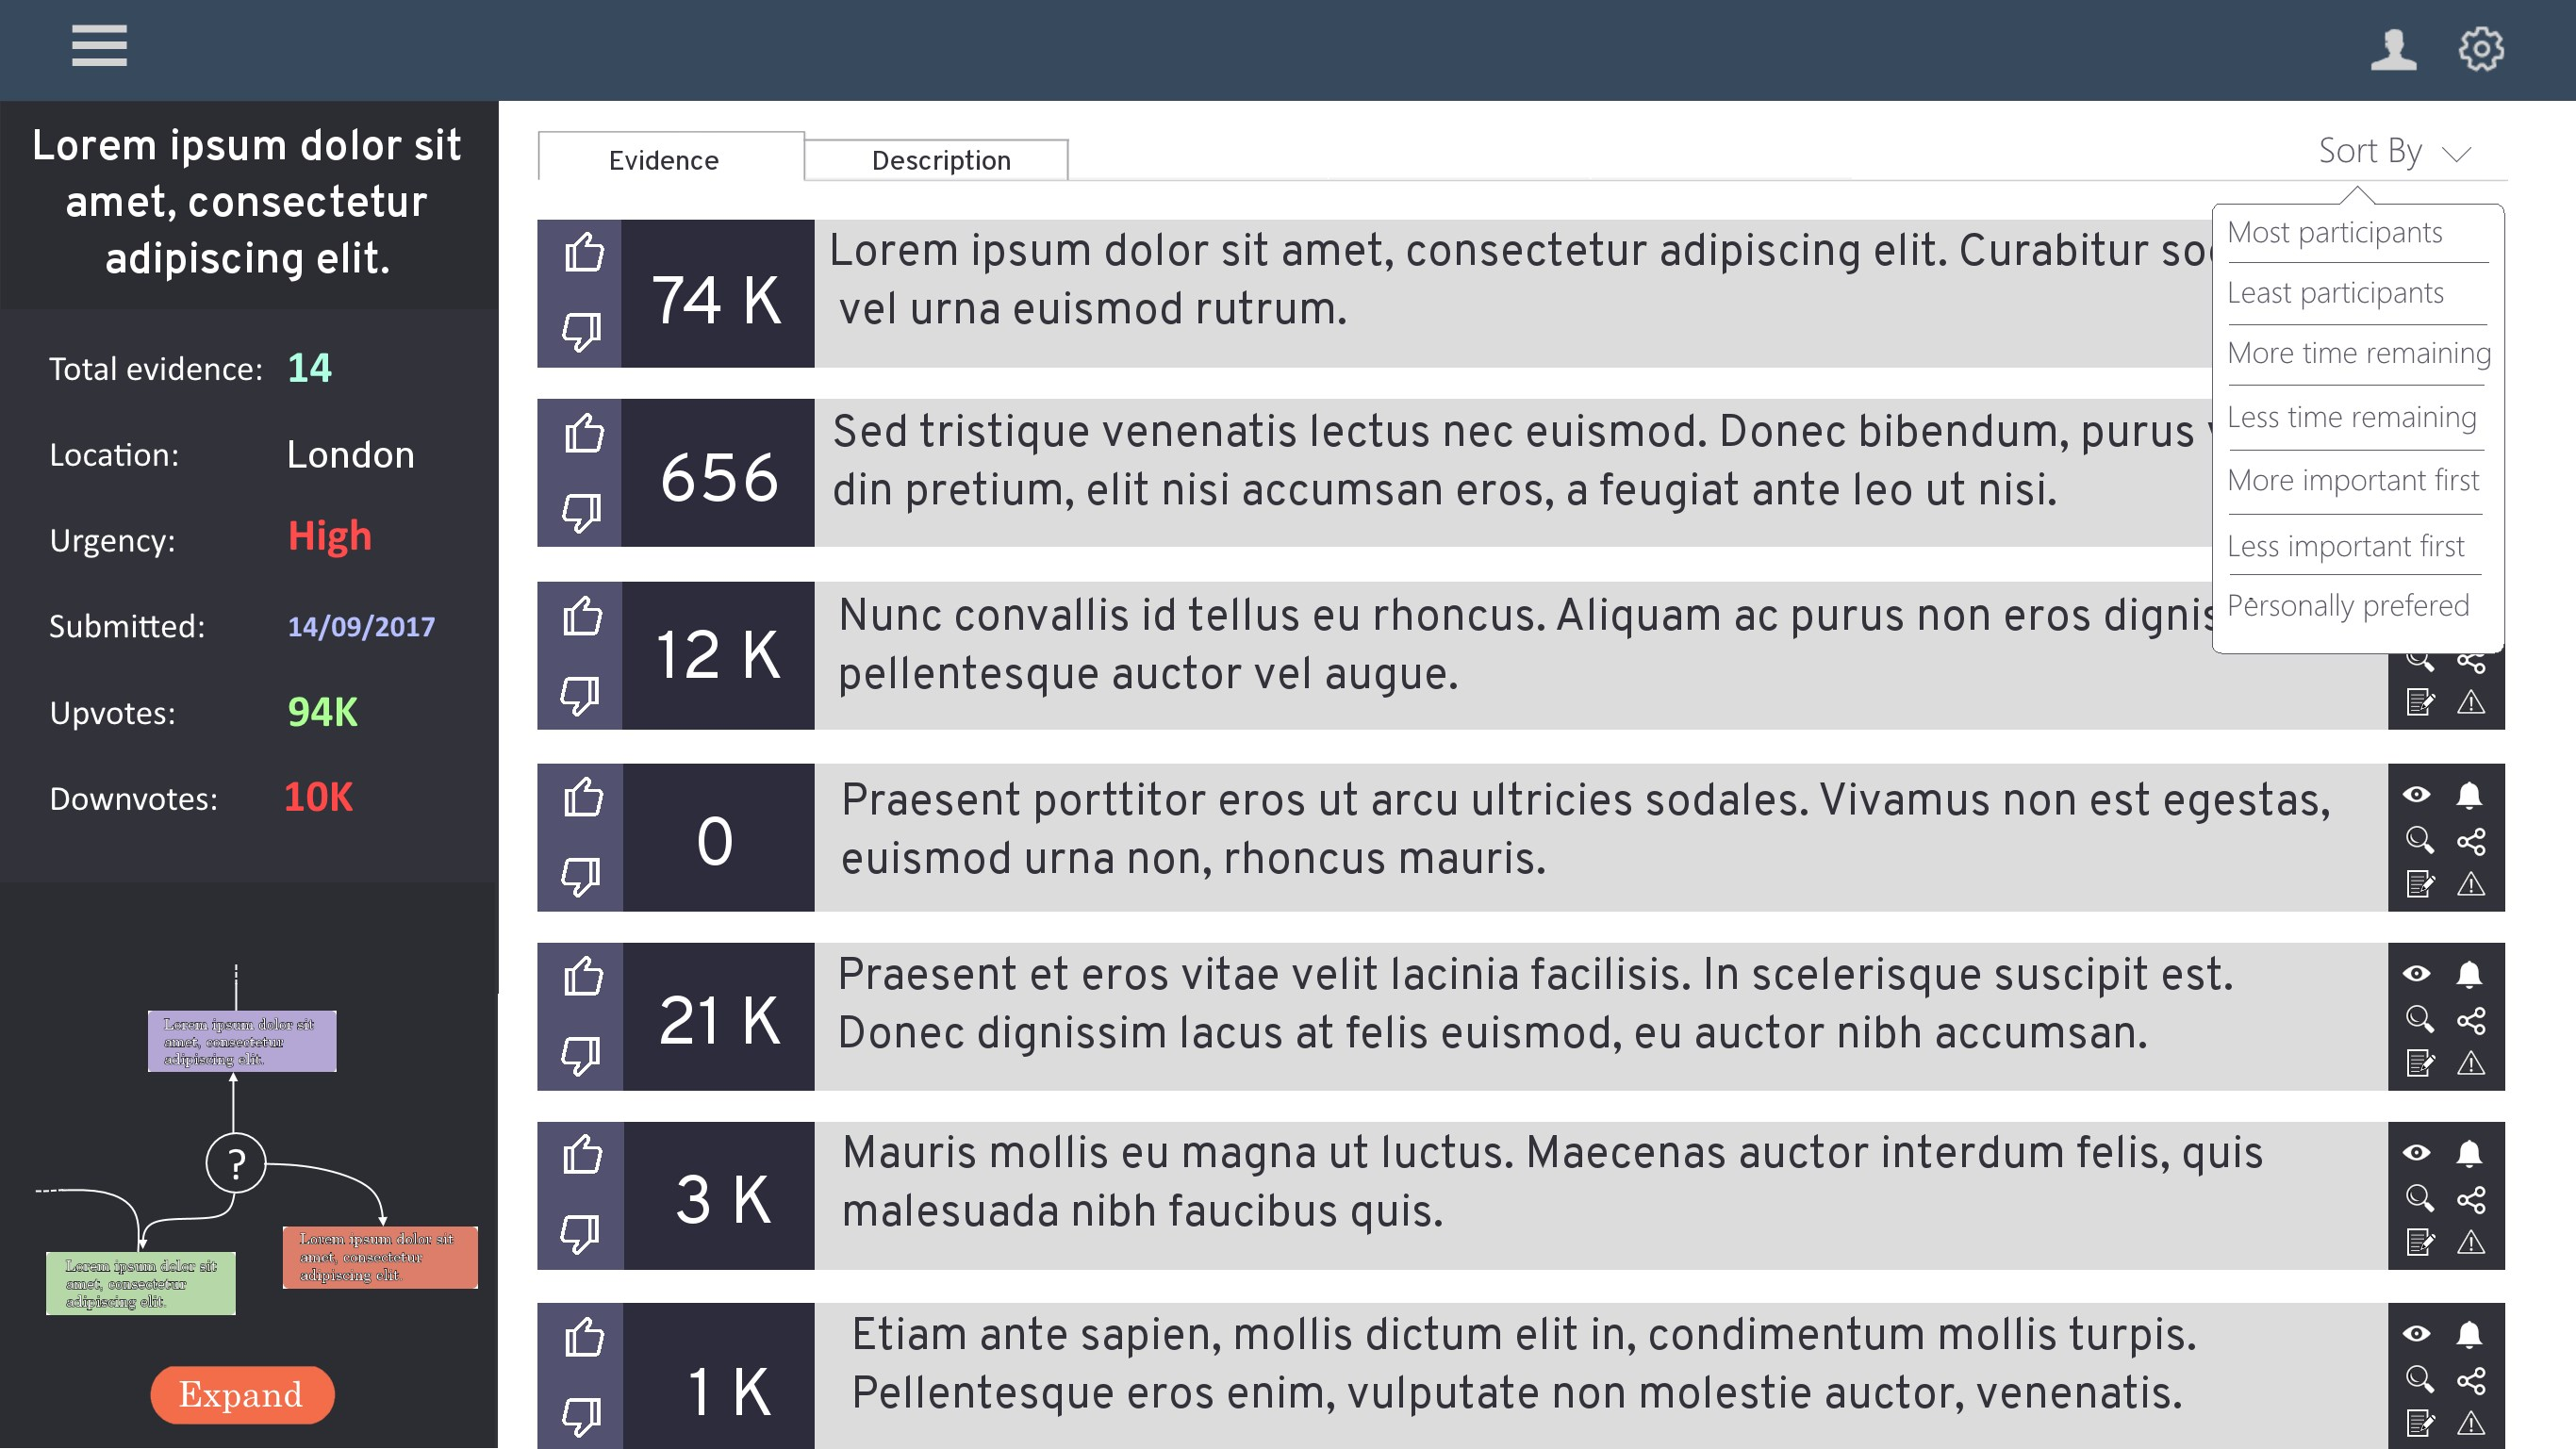
\includegraphics[width=140mm]{FigureA.jpg}
% FigureA.jpg: 2732x1537 px, 72dpi, 96.44x54.25 cm, bb=0 0 2734 1538
\caption{An illustrated concept of the issues portal.}
\label{figure1}
\end{figure*}

\subsection{Favor} \label{favor}

While other elements depend upon the 33-60 principle to be considered accepted, proposals are supported by favor. Favor is a subsystem that enables a user to support a proposal, but unlike upvotes, users can award favor a \{limited\} number of times in a cycle. A user is unable to give more favor if they reached their limit, until a prior one is unassigned. Proposals need to be favored by at least \{20\%\} of the \{active\} population, to get promoted to the next cycle level.

\subsection{Active population} \label{active}

The active population is assessed every \{10 minutes\}, and the requirements for the participation threshold \{are\} altered accordingly. Upvotes from users who have logged off have a grace period of \{1 hour\} while being considered active. Additionally, every \{10 minutes\} the rate of capital renewal is altered according to the active population in each cycle level.

\section{Submission types} \label{submissiontypes}

\subsection{Issues} \label{issues}

If a user wishes to create an issue, they must also submit evidence. The initial submission of evidence is the one that creates the issue itself. The title of the issue and its description are automatically adopted from that submission.

Issues have their own Cycles and Capital subsystems, and submissions are only possible in the bottom cycle level. Issues can be upvoted or downvoted and if they achieve \{33-60\}, they get promoted to the next cycle level where a larger population percentage is contained. In its default appearance, the Issues subsystem can be seen in Figure \ref{figure1}.

If an issue cannot achieve \{33-60\}, its score simply serves for ranking purposes relative to the other issues within that cycle. If an issue gets promoted to a new level, its score is \{reset\}, meaning it has \{0\} upvotes, \{0\} downvotes, and \{0\%\} participation, and it will rely on the support of the users in that new cycle to get promoted again. If an issue reaches the top cycle level and receives adequate support, it is then exhibited to the entire population.

Issues can be subjected to categorization and be assigned tags that indicate the categories in which they belong to. The tags assigned to the issue are adopted by the tags assigned to the top \{5\} evidence of that issue. The number and the type of those categories are configurable. In that way, a user can search for issues that fall under a certain category.

\subsection{Evidence} \label{evidence}

Evidence is information that can be added to an issue to enrich the knowledge about it, or update it in the event of new information. Evidence can be submitted directly inside an issue, without a Cycles subsystem. However, spending of submission capital \{is\} required, with the renewal rate being adjusted according to the \{total active users\} of the cycle that the issue is currently in. Users can still upvote and downvote evidence purely to show support and rank the most valid or crucial.

Evidence submissions feature a list of questions that describe the incident or problem. The default questions, although configurable, are the following:

\begin{itemize}
\item What has happened?
\item Why is it important?
\item Who has been affected?
\item How and why did it happen?
\item Where did it occur?
\item When did it occur?
\item How much is the cost?
\item How long did it last?
\end{itemize}

In each question, attachments of various types (picture, PDF etc.) \{can\} be added to support the claims of the user. Under each evidence submission, any user is able to insert comments, while replies to those comments will be nested underneath.

\subsection{Duplicates} \label{duplicates}

In the case of an emergency, there is a high probability that many users will submit the same issue and quite possibly the same evidence.

Duplicate detection is administered by user reports. The report of only \{1\} user is required to trigger a duplication check and display a voting, thus enabling the community in that specific cycle to decide if the two elements are indeed duplicates. Upon triggering, the two elements move next to each other and an arrow is drawn with a voting option. The confirmation and the subsequent merging of duplicates is achieved by \{33-60\}. At a later time, if the community decides that the two or more elements are not duplicates, a reversal voting can be triggered by report, and its success depends on \{33-60\}.

A subsequent report of duplication, after two elements have failed to achieve \{33-60\}, or were merged and re-separated, has a new triggering threshold requiring the previous number of users multiplied by \{5\}. Using those values, if initially one user triggered a duplication check and failed, it will then require 5 users to re-trigger, and if that fails as well, it will then require 25 users and so on. This also applies to failure of achieving a duplicate separation. This incremental threshold serves to prevent users from continuously trying to sabotage an element they are not in agreement with.

If multiple issues or evidence are merged, the description and title of the highest-voted one is adopted, whereas the rest of the duplicates are stacked within but \{are\} still available for examination or non-duplicate report. If two issues are merged that contained evidence in different levels, everything within them is merged into their respective ones.

\subsection{Reports} \label{reports}

Instead of relying on administrators to operate, supervise, and moderate, the users themselves assist in the correct function of the platform. Not only does this remove the danger of users with elevated privileges abusing their power, it also serves as a user feedback mechanism that improves their reasoning. Submissions of evidence or issues that are inappropriate (e.g. containing profanity) can be reported to the community.

Similar to duplicate checking, only \{1\} user needs to trigger a check against an inappropriate submission and if the community decides the report is invalid, the number of users that are required to re-trigger the check \{increases\}. If an issue or evidence is regarded by the community as inappropriate, it is hidden in a special section at the bottom of the list and a user can reverse report and trigger a check if they think that the issue or evidence has been mistakenly reported or the variables of the situation have changed.

\subsection{Proposals} \label{proposals}

In each issue, an option is given to users to propose solutions. Those solutions are submitted as proposals with their own separate Cycles system. The deliberation process to collectively create a proposal and improve it through consensus is described in the next section. Each proposal features a short, up to \{300\} word, abstract of the text that reflects the purpose of the proposal as well as expected outcomes.

Under the abstract, there is a section containing criteria which addresses a list of questions. The entire proposal is analyzed in those criteria fields, to increase the efficiency of information overview by the readers.

The default criteria, although configurable, are the following:

\begin{itemize}
\item What will change?
\item Why will this change be beneficial?
\item Who will be affected?
\item How will the change be implemented?
\item When will the change be implemented?
\item Where will the change occur?
\item How much are the associated costs and/or expected earnings?
\item How long will the change last?
\item Are there any special requirements? (such as prerequisite changes in existing systems/policies)
\end{itemize}

In each individual criterion, attachments such as pictures \{can\} be added to support the arguments of the user. References to scientific articles or open data can also be added. Users are able to provide feedback to each criterion by clicking on predefined phrases (\{“Biased”, “Needs more work”, “Not enough info”, “I support this”, “I don't support this”, “Unsafe”, “Not inclusive”\}). This provides a feedback mechanism for the strengths and weaknesses of each criterion.

If an issue no longer needs resolving, a user can simply create a proposal that reads “no action required” and if the rest of the community agrees, they can support that in a referendum.

\begin{figure*}[th]
 \centering
 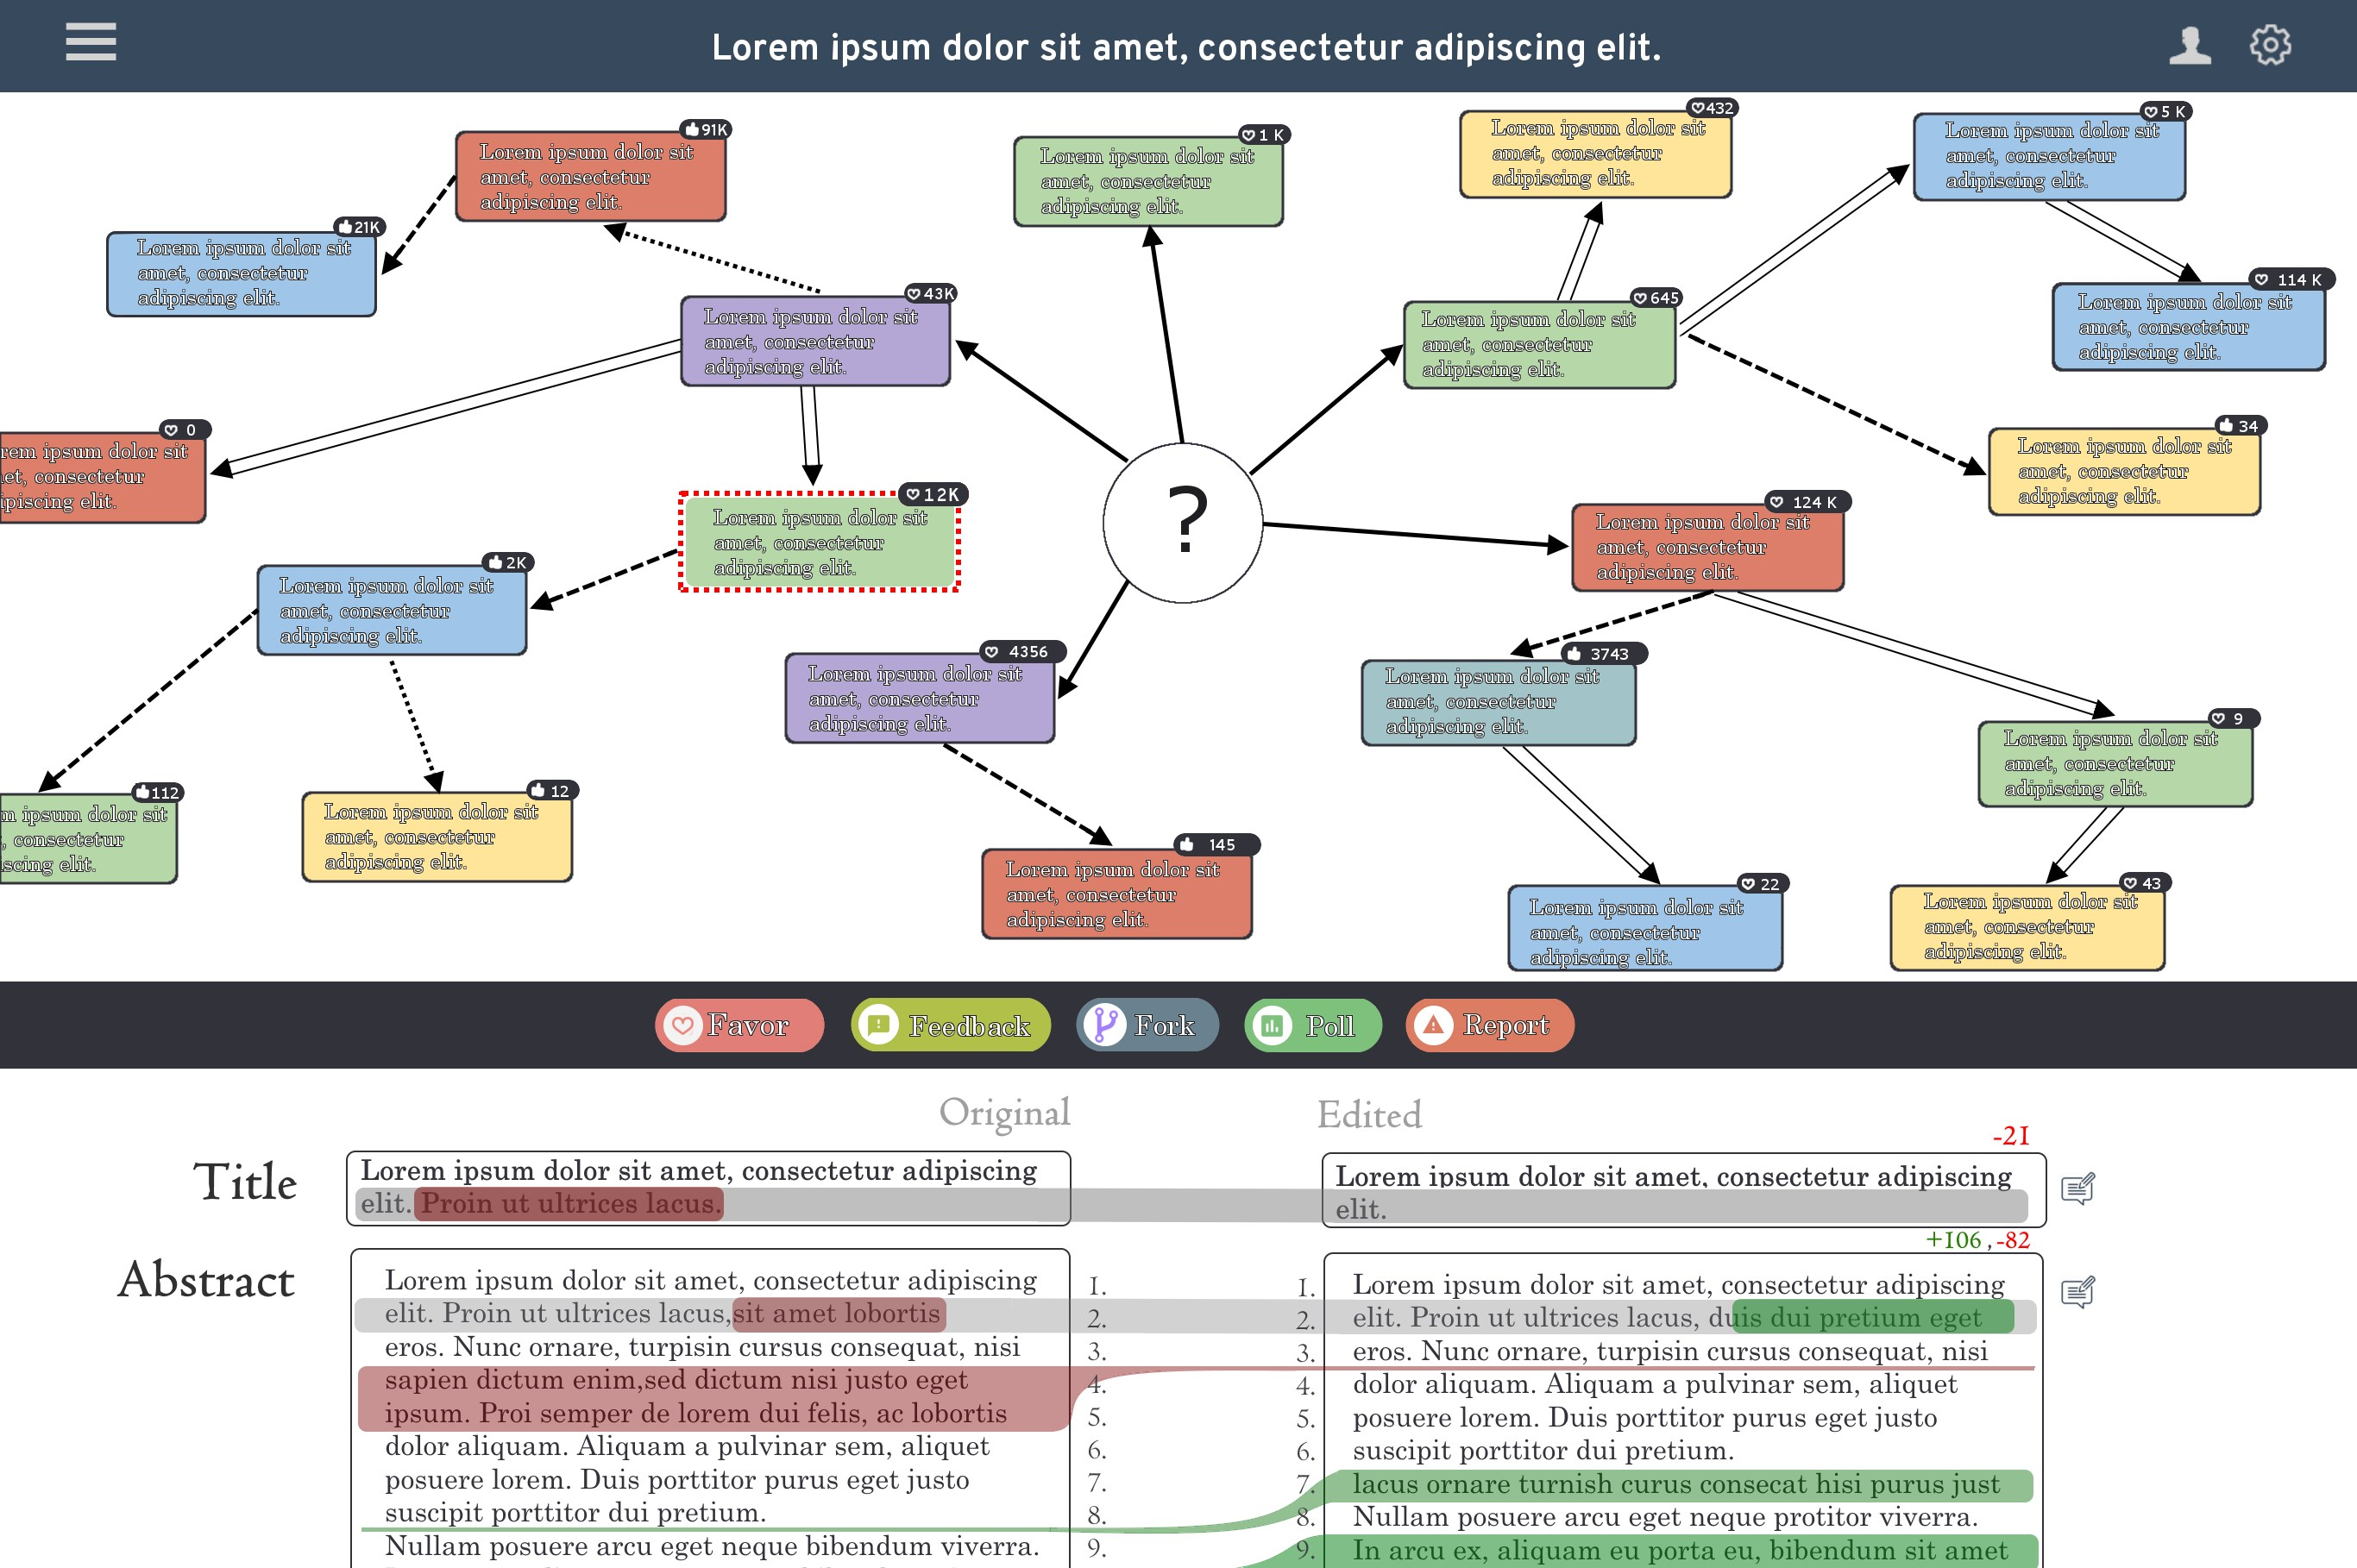
\includegraphics[width=140mm]{FigureB.jpg}
 % FigureA.jpg: 2732x1537 px, 72dpi, 96.44x54.25 cm, bb=0 0 2734 1538
 \caption{An illustrated concept of the deliberation system.}
 \label{figure2}
\end{figure*}

\section{Deliberation} \label{deliberation}

The deliberation section of each issue introduces the user into a tree graph design to enable a fast overview using color and visual cues. Each proposal cycle in each level is a separate map. The main point is a node at the center of a canvas, and different proposals in the form of nodes link to it, creating branches (Figure \ref{figure2}). The different node types in the map are: proposals, forks, feedback and polls (explained below). Each branch further bifurcates as more nodes, forks and feedback are added. The type of link between a node with the previous one indicates the type of the next node.

If two proposals are closely related to one another (or in rare cases even be duplicates) but belong in different branches, it can be reported, and when \{33-60\} is achieved, a “cloud” will be drawn around them to indicate their relevance.

Each node is assigned a unique permalink - a “code” - that a user can reference in other nodes either by text, or simply by clicking another node while they are writing one. Upon detection of a reference towards another node, a link is automatically drawn connecting the two nodes with a single line that will be only visible when clicking the node.

\subsection{Feedback} \label{feedback}

Proposals can only be favored. Instead of having the ability to downvote proposals, users are able to create a “feedback” node. Feedback nodes can be upvoted and downvoted without limits or capital. The content of those nodes is identical to the one in the proposal or fork node they are linked to, but users are able to input additional lines in the original text, denoted by \{gray\} color, that will provide feedback. In that way, they can specify in which exact criterion and line they want to provide feedback to, similar to the in-line comparison of changes in the source of software code.

Users can also report nodes (e.g. containing profanity). In that case, a report node is created, whose contents are a yes-or-no voting. If the voting achieves \{33-60\}, the original node is flagged as inappropriate and it is hidden from the view of users, but there is still the option to view it. A reversal report is possible, although protection against abuse is achieved similarly to the rest of the reports, with the number of users that are required to re-trigger the check \{increasing\} each time.

A feedback node linking to another feedback node cannot be created; users can evaluate feedback nodes simply by upvoting and downvoting them, or reporting them as inappropriate.

\subsection{Forks} \label{forks}

Submitted proposals can be “forked”, which is the ability to take all content from a previous submission (even from a different creator), amend, and resubmit it. A fork could be a revised version of a proposal, in response to a linked feedback node that highlighted weaknesses. The new fork node will contain both the original text and the modified one side by side, and will compensate for the previous proposal's weaknesses by amending its content.

A fork automatically triggers a difference comparison with the previous submission, highlights the added text as \{green\} and the removed as \{red\}, and indicates the number of lines added or deleted for each individual criterion (Figure \ref{figure2}). In that way, the user does not have to read the entire text from the beginning, but they can focus only on the changed one, allowing for fast overview of hundreds of nodes.

\subsection{Polls} \label{polls}

Users are able to create a node that will feature one or more polls. A poll may contain up to \{10\} questions with multiple choices, or input of values through sliders, with the summary statistics (mean, median, standard deviation, quartiles) of all inputs being calculated. Next to each question the agreement as well as the participation are shown as percentages.

\subsection{Promotion} \label{promotion}

Each user has \{3\} instances of favor in each cycle for proposals and forks. If a proposal or a fork node receives favor from more than \{20\%\} of the active population, it is promoted to the next cycle.

Only the top-favored node of a branch is promoted, along with \{33-60\} accepted feedback and \{one-distance\} forks. The node creator \{is also\} promoted to that cycle. That user is now part of two next-level cycles, with separate submission capital and new favor for both of them.

Users must still keep their favor assigned in the lower cycle, and that favor number is now the new baseline of the node in the new cycle. For example, if a user removes their favor in the previous cycle, the favor of the node in the higher cycle would then be -1. Detaching the need to support the node in the previous cycle would allow the users to remove the favor from it and assign it to a new node, thereby allowing them to eventually promote every single node to the next cycle. To prevent that, users in the previous node have to keep their favor assigned.

Once a node is part of new cycle, it still exists in the previous one (even if it ascends to higher levels). Nodes cannot descend to lower cycles. The node, although relying on the lower cycles to maintain its favor, it is separate from them, and new nodes linked to it will not be displayed in the ones below.

\subsection{Visual indications} \label{visual}

Each node has a “score” label in the top-right corner, displaying the number of upvotes and downvotes for feedback and poll nodes, and the number of favor for forks and proposals. 

For an even faster overview, forks and proposals \{are\} colored, with their color indicating the \{amount of favor\} relative to the other nodes in the cycle. The shift of support to an improved fork will also cause changes in the color for both nodes, making the overview of the deliberation easier.

In feedback and poll nodes, the node has always \{white color\}, but the score label is partly \{green\} and partly \{red\}, with each of those two colors occupying areas proportionate to the upvotes and downvotes of the node.

The link type between each node indicates its relationship to the previous one. A \{single line\} indicates reference, a \{dashed line\} indicates feedback, a \{dotted line\} a poll and a \{double line\} indicates a fork to the previous node. The outline type of each node is similar to its link type.

A proposal that was promoted to a higher cycle, has a \{golden\} outline around it.  

\section{Referendums} \label{referendums}

Referendums are proposals which have been widely supported, and are now available for voting by the entire community. For a referendum to be accepted, the required participation level would need to be \{33\%\} of the \{entire\} registered population, not only the currently active one.

If in a top-level cycle a proposal “A” achieves \{20\%\} favor and is therefore ready to convert to a referendum, a check is run through the other top-level cycles to determine if there is another proposal gaining more than \{1\%\} support per \{minute\}. If there is indeed one (or more) proposal “B” that is gaining support fast, it halts the conversion of proposal “A” to a referendum until “B” achieves \{20\%\} favor, in order to introduce them simultaneously as referendums and avoid the problem of a better solution being succeeded by an inferior one, only because it required more time to mature to an adequate level. If more than one proposals are introduced as referendums, the voting mechanism switches from yes-or-no to ranked voting.

If the rate of support of proposal “B” drops under \{1\%\} per \{minute\}, the conversion halts, records the value at which the rate dropped, and re-assesses its rate of support in \{15 minutes\}. Recording the level of support at which the rate dropped is essential, to avoid the exploitation from groups that keep favoring and unfavoring continuously to deliberately sabotage a proposal.

As soon as a referendum has successfully been accepted, it will be indexed in a separate section, so that users will have an available portal to view the policies in effect.

\section{Implementation models} \label{implementation}

\subsection{A global network of academics} \label{academics}

\textit{``Global​ ​Collaboration​ ​against​ ​Global​ ​Challenges''} \\

\noindent{Global challenges are complex in nature, having multiple sources and individual sub-components that constitute and augment them, and span across different fields of knowledge. This means that there cannot be only one authority, but their solution requires the collective effort of thousands of interdisciplinary experts. Moreover, those issues are impossible to solve only on national levels, since change must also happen on an individual level, to be widespread and substantial. Sadly, our current systems of governance do not seem adequately designed to handle those challenges.}

The nature of our challenges is technical, and simply imposing laws does not assist in their solution, it simply modifies human behavior towards them; technical contributions by experts are necessary. For one to be called an expert in a field, not only requires advanced knowledge of the field itself, but also constant contribution to it through the scientific method. Therefore, the individuals who are best fitted to comprehend the depth of the challenges and develop effective and thorough solutions are academics - people who have professorial or research positions at universities.

However, there has not been a way to effectively bring many academics together to provide a space for deliberation, apart from scientific conferences, that still require one to travel to different parts of the world, conducted only once or twice a year, lasting only for a few days and focusing in only one discipline. Collaboration requires thousands and needs to be continuous and asynchronous, thus space, location and time pose serious limitations.

These issues can be well resolved through our platform, as aforementioned, rendering seamless collaboration possible, and that, we believe, is the best possible approach for their solution.

\subsubsection{Operation} \label{operationacademics}

Global issues cannot have a one-size-fits-all approach, due to their numerous underlying causes. Pollution in India may be caused by overpopulation, while in China due to industrial activity. Through a worldwide implementation of our platform, academics will be able to submit issues, tailored to specific regions of the world. Following the report of issues, and their enrichment with evidence, the deliberation section will focus on producing guidelines. Those guidelines would thoroughly explain the course of action towards individuals, local authorities, and national governments. After the most prominent proposals are submitted to referendum, the entire community will vote on what they deem the most viable solution. The deliberation process will be anonymous to ensure that individuals will not be able to bribe academics so as to propose solutions in accordance with their interests.

To address issues in the individual level, a worldwide portal will be created, where each person can view what changes have been recommended for their location and overall lifestyle, as well as how they can help the projects that are being carried out. The guidelines, especially for the individuals, would be summarized in an infographic image. If the issue is of high importance, global crowdfunding campaigns could also be launched to support the cause.

\subsubsection{Establishment} \label{establishmentacademics}

The platform will be hosted on an online server, open for registration by academics. A plugin will be made to verify academic emails and prove academic affiliation. To increase early adoption, apart from recognition, the first successful guideline developments could award a monetary prize to the authors, that would increase the initial interest and boost the overall popularity of the platform. If we were to invite all academic members to register and then actively promote the outcomes, increasingly more academics will be motivated to join.

\subsection{A national decision-making system} \label{national}

Our platform, due to its ability to scale and adapt, could operate as a governance system augmenting or even one day replacing our current representative democracy models. Implemented either locally in small communities, or even nationally, it can dynamically adjust its individual subsystems as described above. The platform could also be integrated along with blockchain technologies to increase the security, remove the reliance on server administrators, and reduce the computational loads or disruptions of service.

\subsubsection{Operation} \label{operationnational}

The subsystem of cycles for issue submission would be ideal for a national model, giving the opportunity to millions of citizens not only to detect and report issues, but also provide ideas for their solution. Issues of technical or complex nature, such as national budget allocation, are challenging for inexperienced citizens. Those issues could obtain joint stands from university boards, laboratories or research centers. Citizens would still have the option to create their own proposals, or operate along a delegative democracy model. In that case, the proposal-making process would be delegated to elected individuals, however everyone in the population could vote on the drafted proposals via a referendum.

By default, citizens will be able to participate in the solution of issues \{only\} in the zones they belong. Although configurable, the default zones that users can participate in, are the municipal, provincial, and national. This means that the issue detection, deliberation and referendums would be specific to different zones, based on each citizen's location.

Public officials would still operate like they do today, carrying out the people's will, similar to how they would carry out the parliamentary decisions in a representative democracy.

In case the solution of an issue requires the development of infrastructure, offers by private contractors will be made, describing in detail the plans and the required funding, and the people will be able to select what they deem the most viable.

\subsubsection{Establishment} \label{establishmentnational}

The problem with the approach of previous projects that tried to introduce citizen participation software for governance, is that they attempted to create a national system with inadequate design. Creating a national platform and enticing the people to use it, has been proven to be unsuccessful time and time again; people do not trust it enough to transition as they have not previously experienced it in their daily lives.

People should be accustomed to participating in the decision-making process in their immediate environments first, so that transitioning to a bigger scale will be smoother, while at the same time the interaction would develop their critical thinking. Our platform can be used initially in small communities or organizations, and then be expanded slowly into larger zones of influence once the users feel comfortable. Moreover, no care was given about the lack of deliberation or the achievement of consensus among thousands of members. Creating a simple voting platform does not inspire participation.

There are multiple features that render the usage of our platform useful for communities and corporations, or wherever there is not sufficient trust in assigning the power to one person or a small group. The decision-making and opinion-sharing processes are meritocratic, with the proposals being cultivated and the best of them selected. It could also work as a poll or evaluation tool, in conjunction with an existing form of management, allowing members or employees to submit issues and provide feedback to proposals created by the managing authority.

The nature of the software, being free and open source will offset development costs to volunteers that wish to improve it for their own communities. To aid the adoption in case a group prefers not to host its own instance, a business model of platform-as-a-service will be implemented, which will charge a fee relative to the size of the community, except if they are non-profit in which case there would be no charge.

In that way, the adoption of the platform as a tool would be widespread due to its valuable features and its ability to seamlessly scale, larger masses of population would use it with more important decisions being made; thus gradually, from the ground-up, it could one day function as a national governance instrument.

\section{Argumentation} \label{argumentation}

\subsection{Core values} \label{core}

Our system ensures equal value for all members and respect for their ability to contribute to their community. Every voice can be heard and evaluated not for its power, but for the quality of its ideas.

The capacity of full anonymity enables users to focus exclusively on the content and not the creator, and therefore each proposal will be judged unbiasedly. This meritocratic way of consensus decision-making, increases trustworthiness and credibility to the process, inspiring each person to confidently contribute opinions. Power is distributed equally among the users, resulting in equal responsibility for one's actions in the system. 

The usage of the platform, apart from its ability to liberate communities from the weaknesses that exist when delegating authority, is constantly enriched with diverse opinions, rendering it fully representative of the group.

\subsection{Decision-making capacity} \label{capacity}

Our governance system can be applied in any community which does not trust assigning the power to an individual or a small group, to avoid abuse of power. It could also work as a poll or evaluation tool, in conjunction with an existing form of management, allowing members or employees to submit issues and provide feedback to proposals created by the managing authority.

The decision-making capacity of the system does not degrade under heavy participation. In contrast, as the operation of the system relies on its members, increased participation improves issue detection, and enriches the problem-solving capacity.

Even though there is no moderation or administration monitoring the process, our system can efficiently handle situations where urgent decisions need to be made. As soon as an issue is reported, the deliberation process does not require fixed time periods to produce a result. Given that a proposal is considered mature and is supported by a representative fraction in each cycle (see section \ref{promotion} of the description), consensus outcomes can be produced in mere hours, even with millions partaking in the deliberation.

Additionally, as analyzed in the description, there are certain mechanisms in place to ensure that the exploitation from malicious actors is detected and eliminated.

\begin{figure*}[hb]
\centering
\resizebox{30mm}{!}{\input{wreath.pdf_tex}}
\label{TDFlogo}
\end{figure*}

\subsection{Effectiveness} \label{effectiveness}

The implementation of a global academic model could be an effective way in addressing global challenges. Due to their advanced expertise, academics are the most capable individuals in identifying them and suggesting the required course of action for their resolution. Through our platform, the deliberation section would efficiently allow them to reach consensus and develop guidelines for governments. Guidelines will also be developed towards individual citizens, magnifying the effectiveness.

\subsection{Resources and financing} \label{resources}

The operational cost of the platform will be virtually zero. The nature of the software, being free and open source will offset development costs to volunteers that wish to improve it for their own communities.

In a global model of academics or in a national governance model, the platform could be also integrated along with blockchain technologies to remove the reliance on system administrators and server hosting. Every user will take part in securing the platform by validating its contents, rendering the database tamper-proof.

\subsection{Trust and insight} \label{trust}

The element of our system that strengthens trust and insight is the free and open source nature of the platform. Anyone can review and verify the code and contribute to the development. In addition, values used for configuration are selected by the users, allowing for complete control of the operational core.

The distributed nature of the blockchain breeds trust, as votes and data do not reside in a single point of failure, vulnerable to intrusion. Only verified changes to this database are allowed, thereby preventing vote manipulation, or disruptions of service.

\subsection{Flexibility} \label{flexibility}

Countries, universities, corporations, unions and in general any form of community, society or group can use the platform as their decision-making tool with a multitude of options. Our platform is not a closed and final product, but a collection of numerous, out-of-the-box options and systems for societies and communities to customize to their accord. All the features of our platform and all its subsystems are optional and configurable and can be activated or deactivated as decided by the people.

Users from one community can also act as developers and add features to the platform, that would also be available and benefit everyone. Different communities will decide which features to enable and how to configure them, by opening an issue and reaching consensus on the preferred value.

\subsection{Protection against the abuse of power} \label{abuse}

Our focus lies on developing a system where small groups would not be able to enforce an undesirable action without the consensus of the larger part of the community. So far, communities of large size were unable to operate without the delegation of their decision-making power, and as a result, the abuse of that power was constant. In our proposed system, abuse of power or bribing are impossible due to the lack of representatives and moderators.

In a global academic model, the large number of users are spread in many countries, making the targeting of them simply impractical. Additionally, their expertise allows them to easily detect and report proposals created to satisfy private interests. Moreover, the anonymity granted to both academics and contractors ensures that bribing cannot occur.

In a national model, the parameters are similar. There would be millions of users, making it impossible to bribe a majority of them, and moreover their great numbers would filter each top proposal multiple times and easily detect fraudulent or deceitful incentives.

\subsection{Accountability} \label{accountability}

The design of our system does not require moderators or an authority of any kind; users themselves have the right and accountability for the operation of the system, since decided outcomes will affect their future. Liability is split evenly among every user, and that increases the feeling of prudence and responsibility, in contrast to today's delegative systems that place the individual in a passive role.

In a global academic model, even though users will need to make a thorough review of the literature before suggesting a solution, their proposals will be checked by multiple peers, and therefore if something is inaccurate, incomplete or contains vested interests, it would be highlighted by simply creating feedback nodes and then forks (as described in section 5 of the description).


\end{multicols}
\end{document}
